\documentclass[10pt]{article}

\usepackage{graphicx}
\usepackage{amsmath}
\usepackage{amssymb}
\usepackage{amsthm}
\usepackage{color}
\usepackage{comment} 
\usepackage{url}
\usepackage[numbers]{natbib}
\usepackage{xcolor}
\usepackage{listings}
\lstset{language=bash,
  basicstyle=\ttfamily\footnotesize,
  showstringspaces=false,
  commentstyle=\color{red},
  keywordstyle=\color{blue}
}

\title{Vector Field K-Means Code}


%%%%%%%%%%%%%%%%%%%%%%%%%%%%%%%%%%%%%%%%%%%%%%%%%%%%%%%%%%%%%%%%%%%%%%%%%%%%%%%%%%%%%%%%%%%%%
%% Document
%%%%%%%%%%%%%%%%%%%%%%%%%%%%%%%%%%%%%%%%%%%%%%%%%%%%%%%%%%%%%%%%%%%%%%%%%%%%%%%%%%%%%%%%%%%%%

\begin{document}

\maketitle

%%%%%%%%%%%%%%%%%%%%%%%%%%%%%%%%%%%%%%%%%%%%%%%%%%%%%%%%%%%%%%%%%%%%%%%%%%%%%%%%
%% SECTION: Introduction
%%%%%%%%%%%%%%%%%%%%%%%%%%%%%%%%%%%%%%%%%%%%%%%%%%%%%%%%%%%%%%%%%%%%%%%%%%%%%%%%
\section{Compiling the Code}
\vspace{0.2cm}
The code has no dependencies, therefore compiling it is very simple. A makefile is
included. In a system in which \emph{make} is available just go to the src directory
in the repository and type make in your terminal. This generates an executable called
\emph{vfkm}. Running this executable with no parameters shows the proper usage as in the
following example

\begin{lstlisting}
./vfkm 
./vfkm trajFile gridRes numVecFields smoothnessWeight outDir
\end{lstlisting}

This shows that the executable receives 5 parameters, described in the following

\begin{itemize}
\item[1.] The \emph{trajFile} parameters is the path to the file containing the trajectory data to be clustered.
this file should be formatted as in section \ref{sec:file_format}.
\item[2.] The \emph{gridRes} parameter is an integer number corresponding to the resolution of the grid used to 
estimate the vector fields.
\item[3.] The \emph{numVecFields} parameter is the number of vector fields (i.e. cluster) to be estimated (computed).
\item[4.] The \emph{smoothnessWeight} parameter corresponds to a real value between 0 and 1 that corresponds to how
important the smoothness of the vector fields is to the optimization (see the Vector Field K-Means paper for more details).
\item[5.] The \emph{outDir} parameter is the path of the directory in which the results of the algorithm are going to be placed.
See section \ref{sec:output_format} for a description of the algorithm output.
\end{itemize}

\section{Running Example}
To illustrate the usage of the code as well as the input and output files we are going to use a concrete example.
Assume that we have a data set composed of 4 trajectories that we want to cluster. These trajectories are given by
the following sequence of space-time points (i.e., the two first coodinates correspond to space coordinates and 
the third coordinate corresponds to time)

\begin{itemize}
\item $\alpha_1 = (0.1,0.2,0) , (0.1,0.5,1)$
\item $\alpha_2 = (0.05,0.6,0) , ( 0.45 , 0.65 , 0.25 ) , ( 0.75 , 0.55 , 0.5 ) , ( 0.95 , 0.6 , 1 )$
\item $\alpha_3 = (0.2,0.1,0) , (0.15,0.5,0.5), (0.25,0.95,1)$
\item $\alpha_4 = (0.4,0.8,0) , (0.5,0.85,0.5), (0.75,0.825,1)$
\end{itemize}

These trajectories are shown in figure \ref{figs:first_example}.

\begin{figure}
\centerline{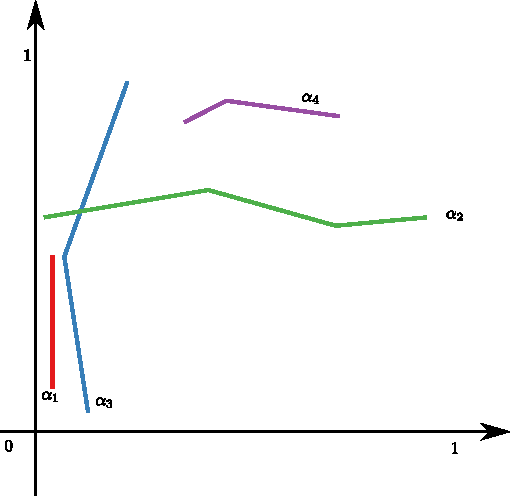
\includegraphics[width=0.5\linewidth]{figs/first_example.pdf}}
\caption{Trajectories in the example.}
\label{figs:first_example}
\end{figure}

\section{Data Input}\label{sec:file_format}
In this section we describe the format of the trajectory file used by the code.
The first line of this file contains the bouding box of the region used to estimate
the vector fields ($\Omega$ in the paper notation). This line follows the format "left right bottom top startTime endTime". After this first line contains the trajectory data. Each line
contains the space time coordinates of the trajectories and distinct trajectories are separated
by a line containing "0.0 0.0 0.0". For example, let's assume that we want to compose the file
containing the trajectories of the previous section and also that we want to estimate
the vector fields in the square $[0,1]\times [0,1]$ and the time bounds are also $[0,1]$.
The result file is the following

\begin{lstlisting}
0 1 0 1 0 1
0.1 0.2 0
0.1 0.5 1
0.0 0.0 0.0
0.05 0.6 0
0.45 0.65 0.25
0.75 0.55 0.5
0.95 0.6 1
0.0 0.0 0.0
0.2 0.1 0
0.15 0.5 0.5
0.25 0.95 1
0.0 0.0 0.0
0.4 0.8 0
0.5 0.85 0.5
0.75 0.825 1
0.0 0.0 0.0
\end{lstlisting}

Let's assume that this file is saved as \emph{trajectories.txt}.
Figure \ref{figs:file_example} highlights the different portions of the file format.

\begin{figure}[!h]
\centerline{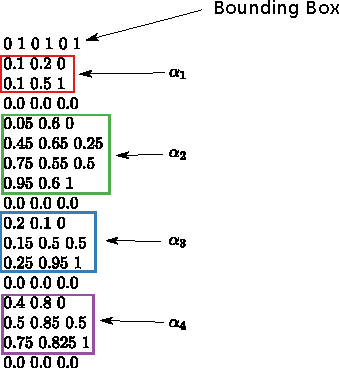
\includegraphics[width=0.75\linewidth]{figs/file_example.pdf}}
\caption{The \emph{trajectories.txt} file example.}
\label{figs:file_example}
\end{figure}

Trajectories not contained in this grid are tesselated. 

\section{Running the Algorithm}\label{sec:running_algorithm}

\begin{figure}[!h]
\centerline{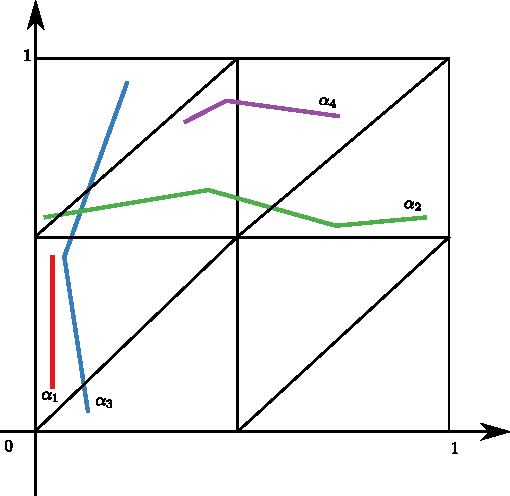
\includegraphics[width=0.5\linewidth]{figs/grid_example.pdf}}
\caption{Grid example.}
\label{figs:grid_example}
\end{figure}

Now we are ready to run the algorithm. Assume that we want to find 2 clusters
(estimate 2 vector fields), using a grid of resolution 3 (i.e., the given bounding box 
is going to be splitted using a triangular grid 18 triangles as in figure \ref{figs:grid_example}), and a smoothness weight
of 0.5. Furthermore, we want the output to be placed in the directory called \emph{finalOutput}.
We do this by

\begin{lstlisting}
./vfkm trajectories.txt 3 2 0.5 finalOutput
Loading Files...
Loading data
CALLING THIS
Optimizing...
Before optimization: 1e+20
After optimization: 0.320979
After assignment: 0.320979 changes: 0
Cleaning Memory
\end{lstlisting}

The output files should now be in the directory \emph{finalOutput}. Let's check!

\begin{lstlisting}
ls finalOutput
curves_r_0.txt  curves_r.txt    vf_r_0.txt  vf_r.txt
curves_r_1.txt  experiment.txt  vf_r_1.txt
\end{lstlisting}

In the following section we describe each of these files.

\section{Algorithm Output}\label{sec:output_format}
The algorithm generates a series of files in the output directory as shown previously.
You should only worry about the \emph{curves\_r\_i.txt} and \emph{vf\_r\_i.txt} files, since
these contains the assingment of curves to clusters and the vector fields. For each $i=0,1,...,$ \emph{numVecFields} (the number of clusters passed as a parameter when the code was run), these
pair of files is going to be created. You should ignore the files \emph{experiment.txt, curves\_r.txt,} and \emph{vf\_r.txt}

\subsection{Curve Files}
The curve files are in the following the format

\begin{lstlisting}
curveIndex error
curveIndex error
...
curveIndex error
\end{lstlisting}

where \emph{curveIndex} corresponds to the index of the curve in the
input file (the order in which the curves were given) and error
corresponds to the residual in the optimization problem corresponding
to that curve. 

As an example, let's look at the curve files generated in the last example. The 
\emph{curves\_r\_0.txt} file is 

\begin{lstlisting}
0 0.00389544
2 0.0980094
3 0.0244096
\end{lstlisting}

This indicates that the curves $\alpha_1, \alpha_2,$ and $\alpha_4$ (indices 0,2, and 3) 
were put in the cluster 0. The file \emph{curves\_r\_1.txt} is

\begin{lstlisting}
1 0.141112
\end{lstlisting}

which indicates that the curve $\alpha_2$ was put by itself in cluster 1.

\subsection{Vector Field Files}

The vector field files contain the estimated vector field. As described in
the Vector Field K-Means papers, vector fields are given by their values in
the vertices of the grid. The vector field files are in the following format

\begin{lstlisting}
numVertices
xComponent yComponent
xComponent yComponent
...
xComponent yComponent
\end{lstlisting}

The first line contains the number $n$ of vertices that are used to define this vector field.
The following $n$ lines contain the values of the vector fields (first the $x$ component and
after that the $y$ component) for each of the vertices starting from the bottom left vertex
in the grid ending in the top right one (going each row at a time from left to right). Figure
\ref{figs:vertex_ordering} illustrates the ordering of the vertices in the vector field files.

\begin{figure}[!h]
\centerline{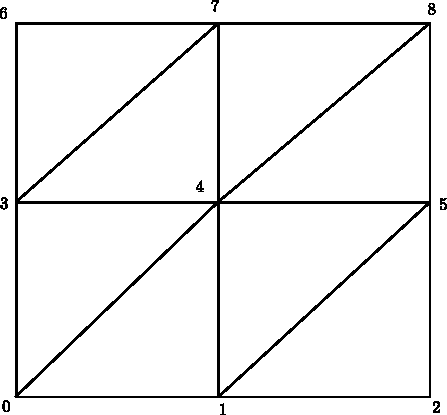
\includegraphics[width=0.5\linewidth]{figs/vertex_ordering.pdf}}
\caption{Vertex ordering.}
\label{figs:vertex_ordering}
\end{figure}

\end{document}
